\documentclass[aspectratio=169]{beamer}
\usepackage{tikz}
\usetikzlibrary{shapes,arrows,positioning}

\begin{document}

\begin{frame}{FNO Class Structure}
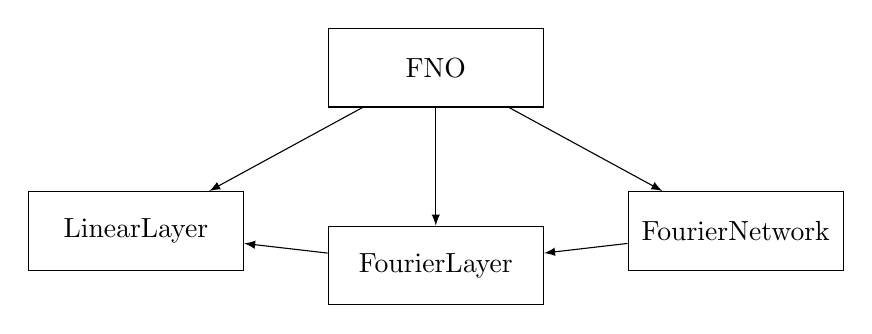
\begin{tikzpicture}[
    node distance=1.5cm,
    block/.style={rectangle,draw,text width=2.5cm,text centered,minimum height=1cm},
    line/.style={draw,-latex}]

    % Main FNO class
    \node[block] (fno) {FNO};
    
    % Component classes
    \node[block, below left=of fno] (linear) {LinearLayer};
    \node[block, below=of fno] (fourier) {FourierLayer};
    \node[block, below right=of fno] (fournet) {FourierNetwork};
    
    % Connect classes
    \path[line] (fno) -- (linear);
    \path[line] (fno) -- (fourier);
    \path[line] (fno) -- (fournet);
    \path[line] (fourier) -- (linear);
    \path[line] (fournet) -- (fourier);
\end{tikzpicture}
\end{frame}

\begin{frame}{Key Parameters}
\begin{columns}
\begin{column}{0.5\textwidth}
\textbf{Hyper Parameters:}
\begin{itemize}
\item p\_1, p\_2, p\_3
\item learning\_rate
\item n\_epochs
\item batch\_size
\item device
\item alpha
\item best\_loss
\end{itemize}
\end{column}

\begin{column}{0.5\textwidth}
\textbf{Fourier Parameters:}
\begin{itemize}
\item n\_layers
\item n\_modes 
\item dim\_coords
\item activation
\item kernel\_initializer
\end{itemize}

\textbf{Regular Parameters:}
\begin{itemize}
\item first\_network
\item last\_network
\item fourier\_network
\end{itemize}
\end{column}
\end{columns}
\end{frame}

\end{document}
